
% Header shows only main title (without "Technical Report" subtitle)
\fancyhead[C]{\footerfont Scalable Training of Mixture-of-Experts Models with Megatron Core}
\maketitle
% Add copyright as unnumbered footnote in the same footnote area
\vspace{-15pt}
\begingroup\renewcommand\thefootnote{}\footnotetext{\par\vspace*{2pt}\textcopyright\, \the\year{} NVIDIA. All rights reserved.}\endgroup
% \vspace{-5pt}
\begin{abstract}
Scaling Mixture-of-Experts (MoE) training introduces systems challenges absent in dense models. Because each token activates only a subset of experts, this sparsity allows total parameters to grow much faster than per-token computation, creating coupled constraints across memory, communication, and computation. Optimizing one dimension often shifts pressure to another, demanding co-design across the full system stack.

\vspace{0.5em}
We address these challenges for MoE training through integrated optimizations spanning memory (fine-grained recomputation, offloading, etc.), communication (optimized dispatchers, overlapping, etc.), and computation (Grouped GEMM, fusions, CUDA Graphs, etc.). The framework also provides Parallel Folding for flexible multi-dimensional parallelism, low-precision training support for FP8 and NVFP4, and efficient long-context training. On NVIDIA GB300 and GB200, it achieves 1,233/1,048 TFLOPS/GPU for DeepSeek-V3-685B and 974/919 TFLOPS/GPU for Qwen3-235B. As a performant, scalable, and production-ready open-source solution, it has been used across academia and industry for training MoE models ranging from billions to trillions of parameters on clusters scaling up to thousands of GPUs.

\vspace{0.5em}
This report explains how these techniques work, their trade-offs, and their interactions at the systems level, providing practical guidance for scaling MoE models with Megatron Core.
\end{abstract}
\abscontent%
% Graphical Abstract - Visual overview of Megatron-Core MoE
\vspace{1ex}
\begin{figure}[H]
    \centering
    \vspace{-0ex}
    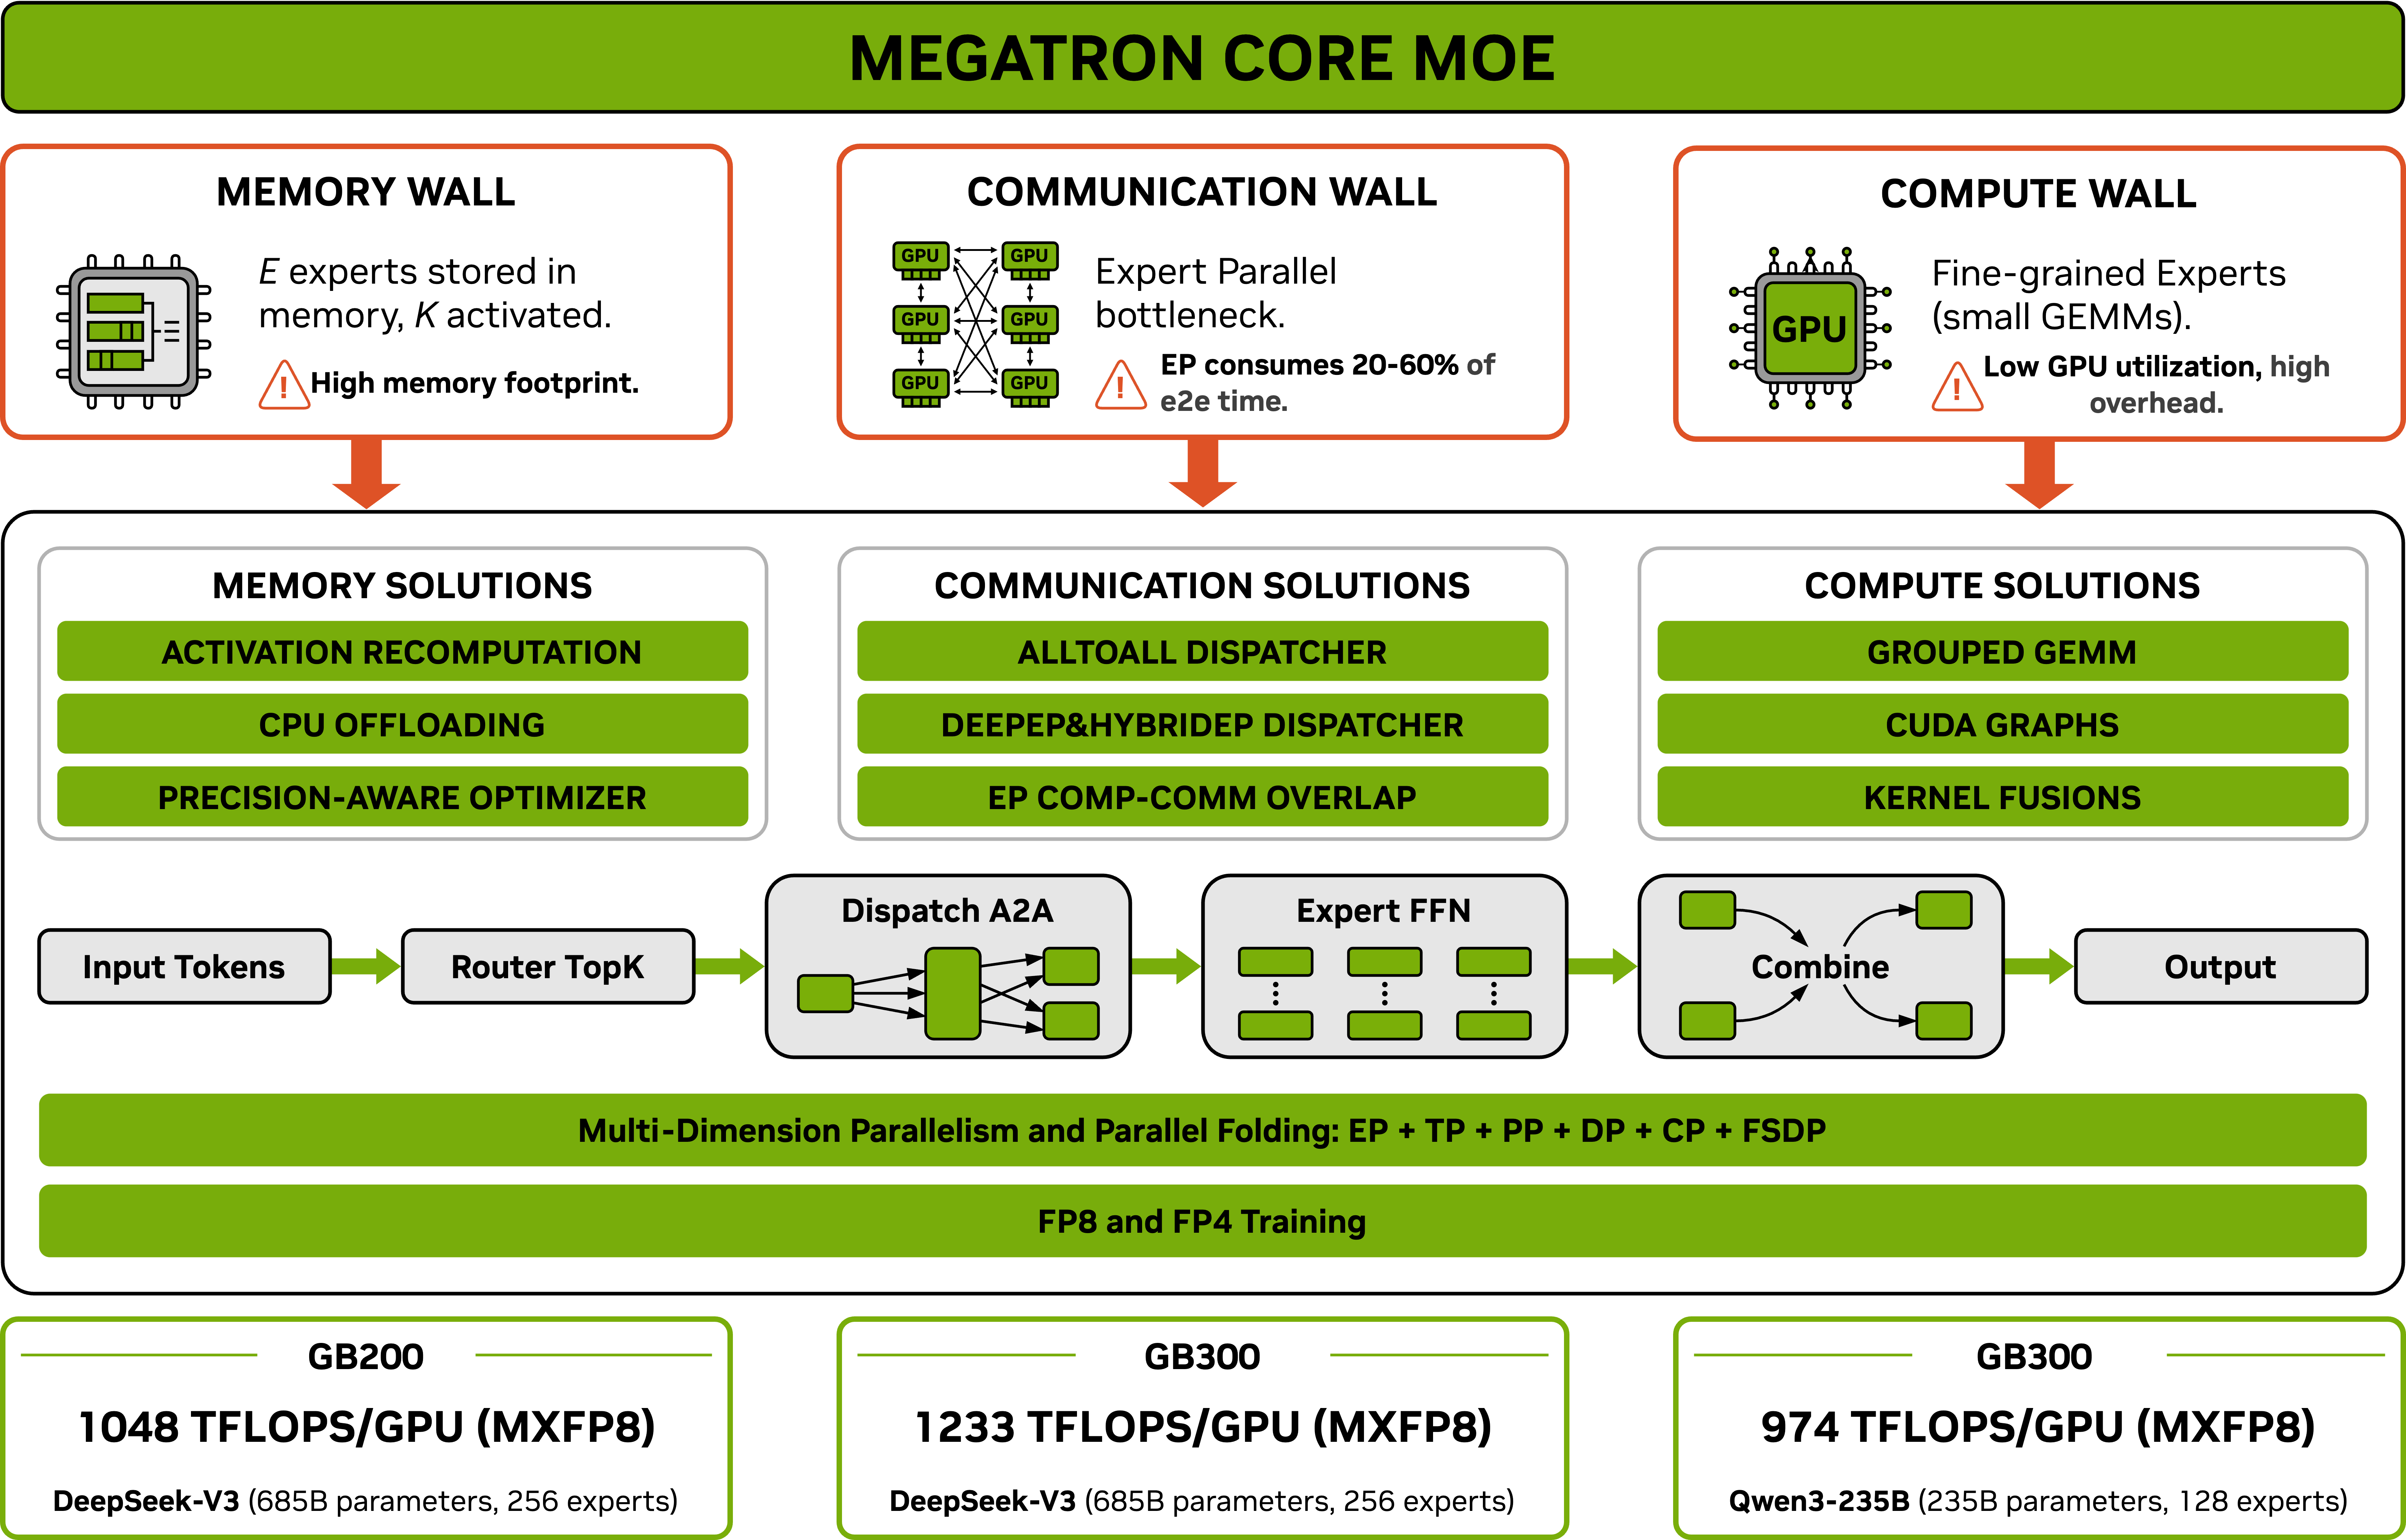
\includegraphics[width=0.93\textwidth,trim=0 0pt 0 2pt,clip]{figures/megatron_core_moe.drawio.png}
    \label{fig:graphical-abstract}
\end{figure}
\vspace{2ex}
\tableofcontents % Add a table of contents
\newpage

\section{Introduction}

Training dense transformers at scale requires computation that grows linearly with model size \cite{kaplan2020scaling,hoffmann2022chinchilla}. Mixture of Experts (MoE) models follow a different scaling pattern: by routing each token to a selected subset of expert networks rather than activating all parameters, per-token computation grows sub-linearly with model size \cite{shazeer2017,fedus2022switchtransformersscalingtrillion}. Recent MoE models have demonstrated order-of-magnitude reductions in training cost relative to quality-matched dense models \cite{jiang2024mixtralexperts,deepseekai2025deepseekv3technicalreport,Cai_2025}.

However, training MoE at scale introduces systems challenges that dense-model frameworks were not designed for. This report presents Megatron-Core MoE, the MoE training stack within Megatron-Core~\cite{shoeybi2020megatronlmtrainingmultibillionparameter}, covering the architecture, parallelism strategies, and system optimizations required to train trillion-parameter-class MoE models at high throughput.

\subsection{Mixture of Experts}

A Mixture of Experts (MoE) model augments a standard neural network with a collection of specialized sub-networks called \emph{experts}, together with a lightweight \emph{router} (or gating network) that dynamically selects which experts process each input \cite{shazeer2017,jacobs1991adaptive,eigen2013learning}. In the context of Transformer-based language models \cite{vaswani2017attention}, MoE layers typically replace the dense Feed-Forward Network (FFN) blocks: instead of a single FFN applied to all tokens, an MoE layer contains multiple FFN experts, and each token is routed to a small subset (e.g., top-$k$) of these experts based on learned routing weights.

Formally, given an input token representation $\mathbf{x}$, the router computes a probability distribution over $E$ experts:
\[
\mathbf{p}(\mathbf{x}) = \text{Softmax}(\mathbf{W}_r \mathbf{x})
\]
The output of the MoE layer is then computed as a weighted combination of the selected experts' outputs:
\[
\text{MoE}(\mathbf{x}) = \sum_{i \in \text{TopK}(\mathbf{p}(\mathbf{x}))} p_i(\mathbf{x}) \cdot E_i(\mathbf{x})
\]
where $E_i$ denotes the $i$-th expert network. This architecture offers three key advantages: model capacity can grow independently of computational cost by adding more experts (\emph{scalable capacity}); only a fraction of parameters activate per token, reducing FLOPs relative to a dense model of equivalent size (\emph{computational efficiency}); and different experts can specialize on different input types (\emph{specialization}). Appendix~\ref{sec:notation} provides a notation reference for all symbols and abbreviations used in this report.

While the concept dates back to the early 1990s \cite{jacobs1991adaptive,eigen2013learning}, the integration of MoE with modern Transformers has driven renewed interest. GShard pioneered distributed MoE training at scale, introducing Expert Parallelism and load-balancing auxiliary losses \cite{lepikhin2020gshard}. Switch Transformer demonstrated that MoE could scale to trillion parameters while maintaining training stability \cite{fedus2022switchtransformersscalingtrillion}. GLaM showed that MoE could match dense model quality at a fraction of the training cost \cite{du2022glamefficientscalinglanguage}. Frameworks including Tutel \cite{hwang2023tutel} and DeepSpeed-MoE \cite{rajbhandari2022deepspeedmoe} further advanced MoE training systems.

MoE adoption has accelerated across research and industry. Mixtral-8x7B showed that open-weight MoE models can match proprietary dense models while reducing inference cost \cite{jiang2024mixtralexperts}. DeepSeek-V2 and DeepSeek-V3 extended this with fine-grained expert architectures, using hundreds of small experts to maximize the capacity-to-compute ratio \cite{dai2024deepseekmoe,deepseekai2024deepseekv2strongeconomicalefficient,deepseekai2025deepseekv3technicalreport}. NVIDIA's Nemotron-3 family~\cite{nvidia2025nemotron3} adopts a hybrid Mamba-Transformer MoE architecture with LatentMoE~\cite{elango2026latentmoe}, trained at scale using Megatron-Core. Scaling law studies confirm that fine-grained MoE achieves favorable compute-optimal trade-offs \cite{krajewski2024scaling,ludziejewski2025jointmoescalinglaws}, accelerating this trend---while amplifying the systems challenges it creates.

\subsection{Challenges in Training Large-Scale MoE Models}\label{sec:challenges}

As models push toward hundreds of experts with smaller individual capacity, the systems challenges of MoE training grow in proportion. These challenges stem from a single root cause: MoE's \textbf{sparsity}---which manifests as a \emph{Parameter-Compute Mismatch} (total parameters far exceeding active computation, this section) and a \emph{Dense-Sparse Mismatch} (attention and MoE layers requiring conflicting parallelism configurations, Section~\ref{parallelism-strategies}).

\textbf{The core asymmetry comes from sparsity.} In a dense transformer, every parameter participates in every training step. A model with $N_{\text{total}}$ parameters requires roughly $6 N_{\text{total}}$ FLOPs per token (forward and backward combined), so parameters and per-token computation scale in lockstep. Splitting the model across more GPUs usually also splits computation in the same proportion, keeping each GPU busy enough that communication overhead stays small.

For MoE, sparsity causes this coupling to break: only $K$ of $E$ total experts activate per token, so per-token computation is roughly $6 N_{\text{active}}$ rather than $6 N_{\text{total}}$, where $N_{\text{active}}$ scales with $K$ while $N_{\text{total}}$ scales with $E$, and $K \ll E$. This creates a fundamental parameter-compute mismatch: compared with a dense model matched on active parameters per token, an MoE model has far more total parameters, often by an order of magnitude. DeepSeek-V3 illustrates this concretely: 685B total parameters but only 37B active per token, an 18$\times$ gap.

With so little computation per token, model partitioning requires more care than for dense models---naively sharding expert matrices (as Tensor Parallelism would) fragments already-small computations, making them even less efficient. Because MoE experts are independent networks, the natural strategy is \emph{Expert Parallelism} (EP): placing different experts on different GPUs, preserving full-size expert GEMMs. EP introduces all-to-all communication to route tokens to their assigned GPUs (Section~\ref{parallelism-strategies} details why EP is preferred and how Parallel Folding addresses the resulting challenges). This parameter-compute mismatch and EP's communication demands together create three tightly coupled challenges---the \emph{Three Walls}---that constrain every MoE training step:

\textbf{The Memory Wall.} All $E$ experts' parameters, gradients, and optimizer states must reside in memory during training, even though only $K$ activate per token. This creates memory pressure far exceeding that of a dense model with comparable per-token compute~\cite{fedus2022switchtransformersscalingtrillion,Cai_2025}. Reducing this pressure requires spending elsewhere: distributing parameters across more devices costs \emph{communication bandwidth}; recomputing activations instead of storing them costs \emph{extra computation}; offloading to host memory costs \emph{PCIe bandwidth}. Dynamic routing further complicates matters: uneven token distributions cause unpredictable memory spikes when some experts receive disproportionate load~\cite{lepikhin2020gshard,wang2024auxiliarylossfreeloadbalancingstrategy}.

\textbf{The Communication Wall.} EP requires all-to-all collectives to dispatch tokens to their assigned experts and collect results~\cite{lepikhin2020gshard}. The per-GPU send volume in each all-to-all is approximately $T \cdot K \cdot h \cdot \frac{EP-1}{EP}$, where $T$ is the local token count, $K$ the top-$k$, and $h$ the hidden dimension; a full dispatch-and-combine cycle doubles this. As EP grows, this volume saturates but the communication increasingly moves from high-bandwidth intra-node links (e.g., NVLink) to narrower inter-node interconnects, where available bandwidth drops by an order of magnitude~\cite{deepep2025}. The sparse activation pattern, meanwhile, provides limited computation to overlap with this communication. In architectures like DeepSeek-V3, where experts span multiple nodes, unoptimized all-to-all can consume up to 60\% of total training time.

\textbf{The Compute Efficiency Wall.} MoE introduces computational inefficiencies absent in dense models:
\begin{itemize}[nosep,leftmargin=*]
    \item \textbf{Small GEMMs.} Fine-grained experts produce many small matrix multiplications that underutilize GPU compute units~\cite{megablocks}. In our measurements, GEMMs account for $\sim$70\% of execution time in Llama-3 405B (dense) but under 50\% in DeepSeek-V3 (MoE). The remainder is consumed by operations that scale with tensor count rather than FLOP count.
    \item \textbf{Routing and permutation overhead.} Token routing and permutation, absent in dense models, add $\sim$9\% to layer execution time even after optimization.
    \item \textbf{Load imbalance.} Dynamic routing assigns uneven token counts to experts, leaving some overloaded while others sit idle, wasting compute capacity~\cite{wang2024auxiliarylossfreeloadbalancingstrategy}.
    \item \textbf{Host overhead.} MoE launches more kernels for the same amount of FLOPs because of sparsity and routing, and each launch carries fixed host-side cost, these add up and leave the GPU idle between kernels. In dropless MoE, dynamic tensor shapes further require costly host-device synchronization.
\end{itemize}

These three walls are tightly coupled: optimizing one often shifts pressure to another. Increasing batch size improves GEMM utilization but amplifies memory pressure and communication volume. CUDA Graphs eliminate host overhead but require static tensor shapes, conflicting with dropless routing. Grouping tokens across experts improves compute efficiency but complicates load balancing. Section~\ref{parallelism-strategies} provides the detailed parallelism analysis underlying EP and Parallel Folding; Section~\ref{key-features-optimizations} presents Megatron-Core's integrated approach to addressing all three walls while managing their interactions.


\subsection{Megatron-Core MoE}
Built within Megatron-Core, a PyTorch-based library for large-scale transformer training~\cite{shoeybi2020megatronlmtrainingmultibillionparameter,paszke2019pytorchimperativestylehighperformance}, this MoE training stack tackles all three walls simultaneously:

\textbf{Multi-Dimensional Parallelism.} Expert Parallelism (EP) integrates with tensor, pipeline, sequence, and data parallelism. MoE Parallel Folding \cite{liu2025moeparallelfoldingheterogeneous} decouples attention and MoE layer configurations, breaking the traditional $\text{EP} \leq \text{DP}$ constraint and enabling configurations tailored to specific model architectures and hardware topologies.

\textbf{Memory Optimizations.} Fine-grained activation recomputation, memory-efficient permutation, precision-aware optimizers, and activation offloading reduce memory footprint without sacrificing throughput \cite{korthikanti2022reducingactivationrecomputationlarge,a2023learningwithdistributedoptimization}. Comprehensive reduced-precision training (FP8 and FP4) support in expert GEMMs, activations, and communication further reduces activation storage while maintaining convergence through selective precision strategies.

\textbf{Communication Optimizations.} High-performance token dispatchers (DeepEP, HybridEP) maximize bandwidth utilization. Communication-computation overlap hides all-to-all latency behind expert computation.

\textbf{Compute Optimizations.} Grouped GEMM kernels, kernel fusion, CUDA Graphs, and sync-free execution address the computational fragmentation inherent in fine-grained MoE architectures.

\textbf{Production Features.} Load balancing strategies, token dropping with capacity control, distributed optimizer and FSDP support, distributed checkpointing with flexible resharding, and upcycling from dense checkpoints enable deployment at scale.
The MoE stack's modular design enables rapid experimentation, while its production-grade optimizations support training from research prototypes to trillion-parameter models~\cite{nvidiamcoremoeuserguide}. This report explains what the stack provides, why key design decisions were made, and how they address MoE training challenges, with practical guidance for configuration and tuning.

\subsection{Structure of This Paper}

The remainder of this report follows a progression from architecture to optimization to evaluation:

\begin{itemize}

\item \textbf{Section~\ref{meg-core-architecture}: Megatron-Core MoE Architecture.}
Introduces Megatron-Core MoE's design in two parts: the internal design of the MoE layer itself (router, token dispatcher, experts) and the four-stage forward pass (route, dispatch, compute, combine), followed by the external design covering integration with the transformer model, parallel process group organization, and optimizer handling for expert parameters.

\item \textbf{Section~\ref{parallelism-strategies}: Scaling MoE with Parallel Folding and Multi-Dimensional Parallelism.}
Examines how MoE's sparsity breaks the parallelism assumptions of dense training, why Expert Parallelism (EP) is needed alongside traditional strategies, and how the resulting dense-sparse mismatch between attention and MoE layers is resolved by MoE Parallel Folding, which decouples their parallelism configurations for flexible, efficient mapping at trillion-parameter scale.

\item \textbf{Section~\ref{key-features-optimizations}: Breaking the Memory, Communication, and Compute Efficiency Walls.}
Presents Megatron-Core MoE's solutions to the three fundamental barriers: the Memory Wall (activation management, recomputation strategies, offloading, distributed parameter storage), the Communication Wall (optimized dispatchers including DeepEP and HybridEP, communication-computation overlap), and the Compute Efficiency Wall (Grouped GEMM, kernel fusion, CUDA Graphs, sync-free execution for dropless MoE).

\item \textbf{Section~\ref{sec:reduced-precision-training}: Reduced-Precision Training in FP8/FP4 for MoE.}
Covers reduced-precision training as a cross-cutting optimization that simultaneously impacts all three walls by reducing activation memory, halving communication volume, and accelerating Tensor Core GEMMs, while presenting strategies for selective precision to maintain training stability.

\item \textbf{Section~\ref{sec:long-context-training}: Long-Context MoE Training.}
Examines how long-context scenarios (16K to 64K+ tokens) fundamentally shift the optimization landscape as attention computation dominates, and presents techniques for managing activation memory growth through Context Parallelism and Tensor Parallelism scaling.

\item \textbf{Section~\ref{sec:production-features}: Production Features.}
Describes operational features for production training: load balancing and token dropping for stable training, distributed checkpointing for parallelism-agnostic resharding, upcycling from dense checkpoints, and integration with multi-token prediction.

\item \textbf{Section~\ref{performance-evaluations}: Performance Evaluation.}
Validates the framework's effectiveness through empirical benchmarks on DeepSeek-V3 and Qwen3-235B across GB200 and H100 platforms, demonstrating the impact of the full optimization stack.

\item \textbf{Section~\ref{sec:best-practices}: Performance Best Practices with DeepSeek-V3 Case Study.}
Provides a systematic workflow for identifying optimal parallelism configurations, validated through a detailed DeepSeek-V3 case study that demonstrates how the optimizations work together to achieve state-of-the-art performance.

\item \textbf{Section~\ref{sec:rl}: Megatron-Core MoE in Reinforcement Learning.}
Addresses the emerging RL post-training paradigm, covering challenges unique to RL workloads (variable sequence lengths, memory offloading, online weight export), Megatron-Bridge integration with popular RL frameworks, and RL-specific optimizations including packed sequence support, dynamic context parallelism, and router replay.

\end{itemize}


\section{Megatron-Core MoE Architecture}\label{meg-core-architecture}

This section presents Megatron-Core's MoE implementation architecture in two parts. We first describe the \textbf{internal design} of the MoE layer itself: its modular components (router, token dispatcher, experts) and the four-stage forward pass that transforms input tokens into output representations. We then examine the \textbf{external design}: how parallel process groups are organized to support distributed execution and how the optimizer handles expert parameters differently from dense layers.

\subsection{MoE Layer Architecture and Forward Pass}\label{sec:moe-layer-architecture}

An MoE layer replaces the dense feed-forward network (FFN) in a transformer block with a collection of expert FFNs, only a subset of which process each token. Megatron-Core implements this through three modular components (a \emph{router} for token-to-expert assignment, a \emph{token dispatcher} for cross-GPU communication, and \emph{experts} for computation) connected through the four-stage forward pass shown in \figref{fig:moe-forward-pass}. This separation of concerns enables independent optimization: the router can be fused into CUDA Graphs without affecting dispatcher logic, dispatchers can be swapped between all-to-all and DeepEP without modifying expert computation, and expert implementations can use different GEMM backends transparently.

\subsubsection{Forward Pass: Route, Dispatch, Compute, Combine}

The MoE layer processes input tokens through four sequential stages:

% Fix the typo in this figure
\begin{figure}[ht]
\centering
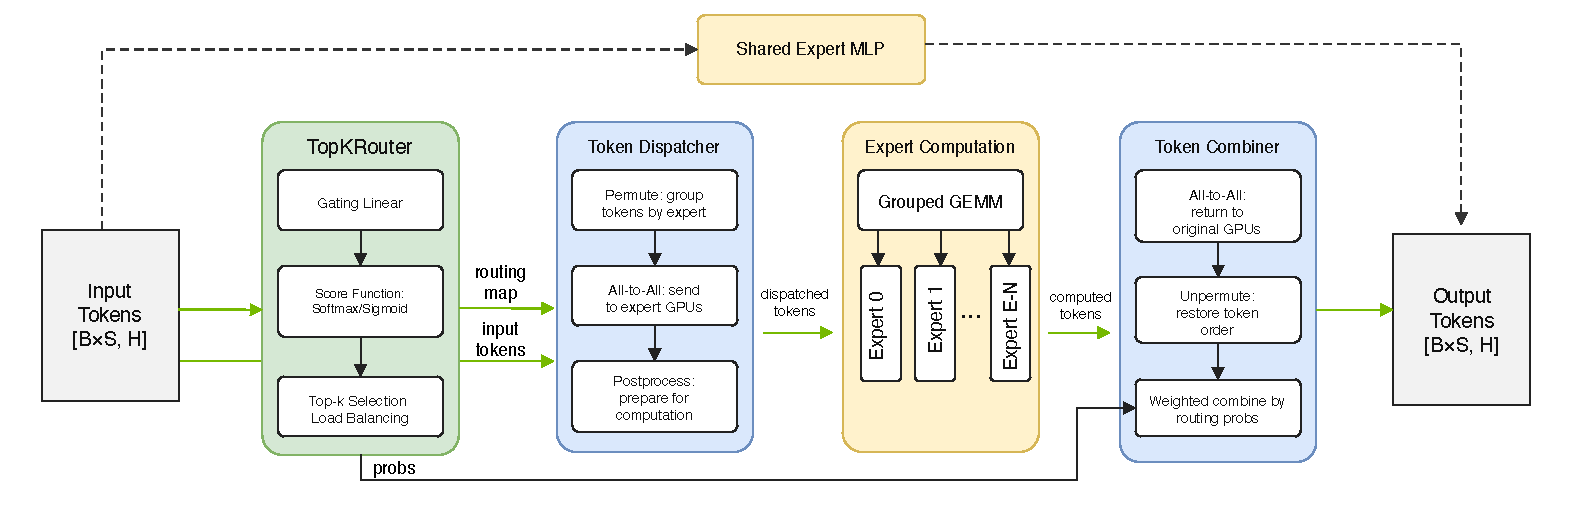
\includegraphics[width=0.9\textwidth]{figures/moe_forward_pass.drawio.pdf} 
\caption{Data flow through an MoE layer: Route, Dispatch, Compute, and Combine stages.}
\label{fig:moe-forward-pass}
\end{figure}

\textbf{Stage 1: Route.} The \texttt{TopKRouter} determines which experts process each token. A learned linear projection maps each token's hidden state to $E$ logits (one per expert), a score function (softmax or sigmoid) converts logits to probabilities, and top-$k$ selection identifies the highest-scoring experts for each token. The router outputs two tensors: \texttt{probs} containing the routing weights, and \texttt{routing\_map}, a boolean mask indicating token-expert assignments. For numerical stability with many experts, the router can operate in FP32 via \texttt{-{}-moe-router-dtype fp32}.

\textbf{Stage 2: Dispatch.} The token dispatcher prepares tokens for cross-GPU communication. It first permutes tokens so that all tokens destined for the same expert are contiguous; this permutation is essential for efficient dense GEMM on the expert side. The dispatcher then moves tokens to the GPUs hosting their assigned experts using one of three backends: AllGather (simple but memory-intensive), all-to-all (standard NCCL-based), or Flex (supporting optimized backends like DeepEP and HybridEP).

\textbf{Stage 3: Expert Computation.} Each GPU executes its local experts on the received tokens. All local experts run in a single Grouped GEMM call via \texttt{TEGroupedMLP}, maximizing GPU utilization even when individual expert workloads are small.

\textbf{Stage 4: Combine.} The inverse communication returns processed tokens to their original GPUs, followed by unpermutation to restore the original sequence order. If a shared expert is configured, its output (optionally computed in parallel with routed experts) is added at this stage.

\subsubsection{Router: Token-to-Expert Assignment}

The router transforms a global token batch into expert-specific workloads through two operations \cite{shazeer2017}:

\begin{enumerate}
    \item \textbf{Gating:} A linear projection $\mathbf{W}_r \in \mathbb{R}^{h \times E}$ maps each token's hidden state $\mathbf{x} \in \mathbb{R}^h$ to logits $\mathbf{l} = \mathbf{W}_r^\top \mathbf{x} \in \mathbb{R}^E$.

    \item \textbf{Top-$k$ Selection:} A score function converts logits to probabilities: softmax ($p_i = e^{l_i} / \sum_j e^{l_j}$) or sigmoid ($p_i = \sigma(l_i) / \sum_j \sigma(l_j)$, used by DeepSeek-V3 \cite{deepseekai2025deepseekv3technicalreport}). The top-$k$ experts with highest probabilities are selected per token.
\end{enumerate}

\begin{figure}[ht]
    \centering
    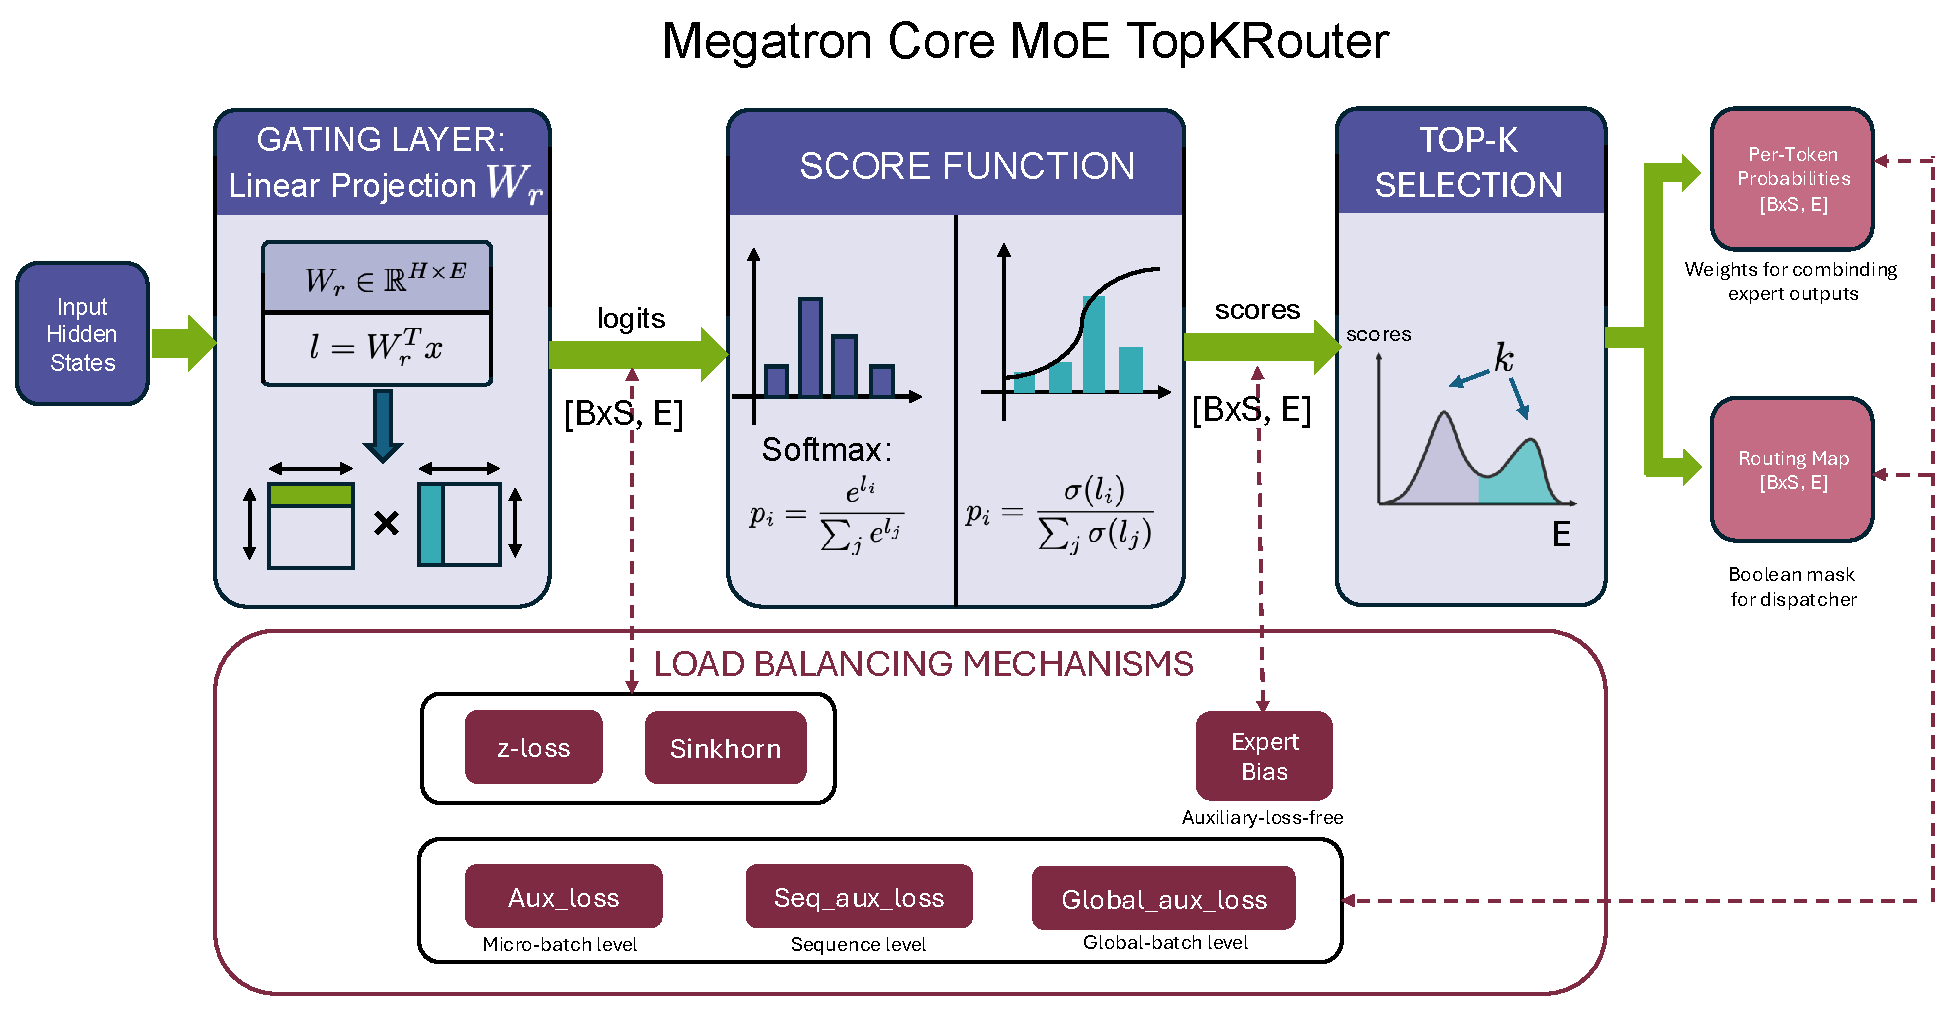
\includegraphics[width=0.85\textwidth]{figures/router.pdf}
    \caption{Router architecture: linear projection, score function, top-$k$ selection, and load balancing.}
    \label{fig:router-architecture}
\end{figure}

Uneven expert utilization degrades both training efficiency and model quality. As shown in \figref{fig:router-architecture}, Megatron-Core supports multiple load balancing strategies; these are discussed in Section~\ref{sec:production-features}.

\subsubsection{Token Dispatcher: Communication Abstraction}

The dispatcher manages token movement between GPUs through a six-phase pipeline: \texttt{dispatch\_preprocess} $\rightarrow$ \texttt{token\_dispatch} $\rightarrow$ \texttt{dispatch\_postprocess} (forward), and \texttt{combine\_preprocess} $\rightarrow$ \texttt{token\_combine} $\rightarrow$ \texttt{combine\_postprocess} (backward).

\textbf{Communication Backends.} Three dispatcher types are available:
\begin{itemize}
    \item \textbf{AllGather} (\texttt{allgather}): Each GPU gathers all tokens and filters for local experts. Simple but memory-intensive; suitable for small EP sizes.
    \item \textbf{All-To-All} (\texttt{all-to-all}): Standard NCCL-based point-to-point communication \cite{lepikhin2020gshard}. Each GPU sends only the tokens needed by each destination. Scales well but incurs synchronization overhead.
    \item \textbf{Flex} (\texttt{flex}): Unified design supporting DeepEP (only high-throughput kernels are integrated, hiding NVLink communication latency through overlap) \cite{deepep2025} and HybridEP (high-bandwidth MoE communication kernels that deliver better performance on NVLink-rich topologies like NVL72).
\end{itemize}

\subsubsection{Experts: Computation Module}

Each expert is a two-layer MLP with optional gating (for SwiGLU/GeGLU activations \cite{shazeer2020glu}). Grouped GEMM enables efficient batching of multiple expert computations \cite{megablocks,hwang2023tutel}. Two implementations are available:

\begin{itemize}
    \item \textbf{TEGroupedMLP}: Transformer Engine \cite{nvidia_transformer_engine} optimized implementation supporting FP8 and FP4 quantization.
    \item \textbf{SequentialMLP}: Executes experts one at a time in a loop. Useful for debugging but significantly slower.
\end{itemize}

\textbf{Shared Experts.} Some architectures (DeepSeek-V2/V3 \cite{deepseekai2024deepseekv2strongeconomicalefficient,deepseekai2025deepseekv3technicalreport}, Qwen \cite{qwen2025qwen25technicalreport}) include a shared expert that processes all tokens regardless of routing. Shared expert computation can run in parallel with the dispatch-compute-combine pipeline, hiding its latency. See Section~\ref{sec:production-features} for details.


\subsection{System Integration: Parallelism and Optimizer}\label{sec:moe-system-integration}

Having described how an MoE layer works internally, we now examine how it integrates into the distributed training system: parallel process groups and optimizer handling.

\subsubsection{Parallel Group Management}

MoE layers require distinct process groups from dense layers because different components have different communication patterns. Megatron-Core organizes these groups through \texttt{ProcessGroupCollection}:

\begin{lstlisting}
ProcessGroupCollection
|-- Attention Layer Groups: tp, cp, dp, pp
|-- Expert Layer Groups:    ep, expt_tp, expt_dp, pp
\end{lstlisting}

Each MoE component uses specific groups based on its communication requirements:

\begin{table}[ht]
\centering
\begin{tabular}{lll}
\toprule
\textbf{Component} & \textbf{Groups Used} & \textbf{Reason} \\
\midrule
Router & \texttt{tp}, \texttt{cp}, \texttt{tp\_cp} & Weights duplicated across EP ranks \\
Token Dispatcher & \texttt{ep}, \texttt{tp\_ep} & all-to-all across expert ranks \\
Experts & \texttt{ep}, \texttt{expt\_tp}, \texttt{expt\_dp} & Sharded across EP; gradients reduced in EDP \\
Shared Experts & \texttt{tp} & Same as dense MLP \\
\bottomrule
\end{tabular}
\caption{MoE component to process group mapping.}
\label{tab:moe-process-groups}
\end{table}

This separation enables \textbf{Parallel Folding} (Section~\ref{sec:parallel-folding}): attention and MoE layers can use different TP/DP configurations. For example, attention layers might use TP=4 while MoE layers use ETP=1 with higher EP, optimizing each layer type independently.

\subsubsection{Optimizer and Gradient Handling}

Expert parameters require distinct handling in distributed optimization. Megatron-Core uses a \texttt{Chained\-Optimizer} that wraps separate optimizers for dense and expert parameters. Three key design decisions support correct MoE optimization:

\begin{enumerate}
    \item \textbf{Parameter Identification.} Expert parameters are marked with \texttt{allreduce=False}, distinguishing them from dense parameters that use standard data-parallel gradient reduction.

    \item \textbf{Separate Reduction Groups.} Dense layers reduce gradients across \texttt{dp\_cp\_group} (full data parallelism), while experts reduce across \texttt{expt\_dp\_group} (expert data parallelism). This ensures gradients are averaged over the correct number of replicas.

    \item \textbf{Gradient Scaling.} Expert gradients are scaled by \texttt{edp\_size / dp\_size} to account for the different effective batch sizes seen by experts (which process routing-dependent token subsets) versus dense layers.
\end{enumerate}

This design allows ZeRO-style optimizer state sharding \cite{rajbhandari2020zero} to work seamlessly with MoE: optimizer states for expert parameters are sharded across the EP group, while states for dense parameters follow standard DP sharding.

With the architecture established, Section~\ref{parallelism-strategies} addresses how to distribute it across devices, and Section~\ref{key-features-optimizations} tackles the memory, communication, and compute efficiency challenges that arise at scale.

\section{Scaling MoE: Parallel Folding and Multi-Dimensional Parallelism}\label{parallelism-strategies}

Section~\ref{sec:challenges} established that MoE's sparsity decouples model size from per-token computation, creating a parameter-compute mismatch that makes Expert Parallelism (EP) necessary but introduces all-to-all communication. This section examines how that mismatch concretely affects parallelism design. We first review the parallelism baseline for dense models and the trade-offs it entails, then show how MoE's sparsity breaks the assumptions underlying these strategies. Finally, we present \textbf{MoE Parallel Folding}, Megatron-Core's solution to the resulting \emph{dense-sparse mismatch}: attention and MoE layers have conflicting optimal parallelism configurations, and Parallel Folding decouples their mappings so each can use its optimal topology.

%==============================================================================
% 3.1 Opening: Why Parallelism, and Why MoE is Different
%==============================================================================
\subsection{Why Parallelism, and Why MoE is Different}\label{sec:why-parallelism}

Before examining MoE-specific challenges, we establish the fundamental reasons parallelism is necessary for large model training and the trade-offs it introduces.

\subsubsection{Why Large Model Training Needs Parallelism}

\textbf{Memory is the fundamental constraint.} A single GPU has limited memory, but training a large model requires storing model parameters, optimizer states, gradients, and activations simultaneously \cite{rasley2020deepspeed}. Consider Llama-405B \cite{grattafiori2024llama3herdmodels,touvron2023llama,touvron2023llama2} trained with BF16 precision and Adam optimizer:

\begin{center}
\begin{tabular}{lr}
\toprule
\textbf{Component} & \textbf{Memory (Llama-405B, BF16)} \\
\midrule
Model parameters & $\sim$810 GB \\
Optimizer states (Adam) & $\sim$4860 GB \\
Gradients & $\sim$1620 GB \\
Activations (8K sequence) & $\sim$5575 GB \\
\midrule
\textbf{Total} & \textbf{$\sim$12865 GB} \\
\bottomrule
\end{tabular}
\end{center}

This far exceeds any single GPU's capacity. Multiple GPUs are not optional; they are \emph{required} to hold the model.

\textbf{Compute throughput is the efficiency reason.} Beyond memory, a single GPU has limited compute capacity. Large model training requires astronomical FLOPs; aggregating multiple GPUs increases throughput and reduces wall-clock training time from years to weeks.

\subsubsection{The Trade-off of Parallelism}

Parallelism is not free. Every parallelism strategy introduces overhead:

\begin{itemize}
    \item \textbf{Communication overhead}: Data exchange between GPUs consumes time and bandwidth.
    \item \textbf{Synchronization}: Fast GPUs must wait for slow GPUs at synchronization points.
    \item \textbf{Pipeline bubbles}: Pipeline parallelism introduces idle time at pipeline boundaries.
    \item \textbf{Reduced compute intensity}: Sharding reduces per-GPU matrix sizes, lowering GEMM efficiency.
\end{itemize}

The result: Model FLOP Utilization (MFU) is heavily influenced by parallelism strategy, and effective parallelism design can minimize the gap between ideal and actual MFU.

\textbf{Key insight for dense models}: The ``cost'' and ``benefit'' of parallelism scale proportionally. More parameters require more GPUs, but more parameters also mean more computation per forward-backward pass. Because computation grows with model size, communication takes a smaller share of each step, keeping MFU relatively stable as models scale.

MoE's sparsity disrupts this balance. Because only $K$ of $E$ experts activate per token, total parameters scale with $E$ while per-token compute scales only with $K$. More GPUs are needed for memory, but per-token computation does not grow to match, leaving communication overhead exposed. The following section examines how this asymmetry breaks the assumptions underlying traditional parallelism strategies and why a new parallelism dimension is needed.

%==============================================================================
% 3.2 The Challenge of MoE Parallelism
%==============================================================================
